\newpage
\section{Method}
% \textit{
% This system was thought of as a tool to be used in many different projects. Because of this the mark on accessibility was big. The developer should not be constrained on what framework or lack there of he or she is using. This should work on all platforms.
% }

This section will present the methods used to answer the research questions (see section \ref{sub:Objective}).  At the beginning of the project, a literature study was performed. This was done to get an overview of similar work in the field. Knowit, the company connected to the study, wanted an easier way to create components for web development projects. A tool was built to fulfill this need. 


Throughout this process, Knowit was involved with semi-weekly checkups for support. Semi-Structured interviews were carried out on the employees of Knowit to steer the development of the tool to fit their needs. 

When a prototype was functional, iterations of usability testing were performed. This was done to ensure that the tool was usable for more people than just the author. Lastly, to investigate what impact the created tool could have, an A/B test was designed.

These steps is shown in figure \ref{fig:projectFlowChart} below.


\begin{figure}[H]
  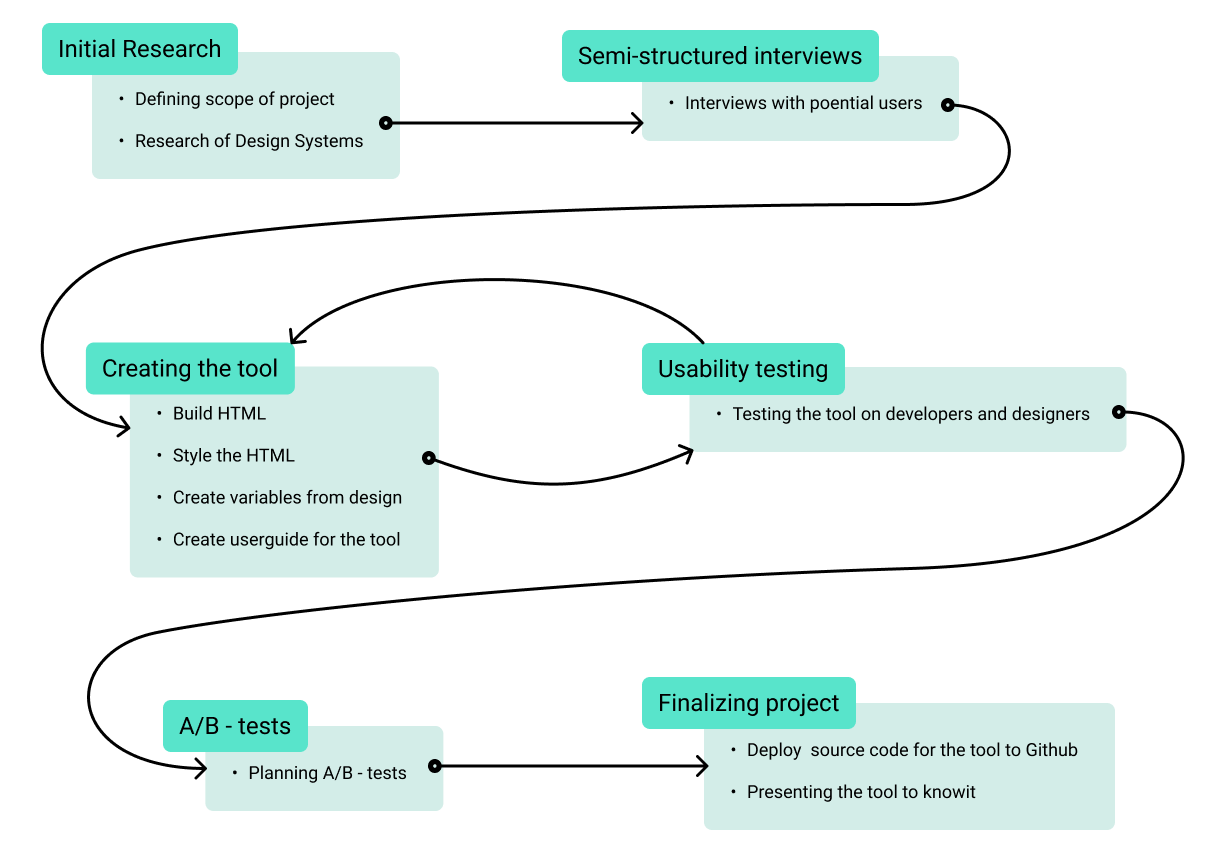
\includegraphics[width=\linewidth]{../images/Project flow chart.png}
  \caption{Flowchart for the project}
  \label{fig:projectFlowChart}
\end{figure}

\newpage
\subsection{Initial Research}%
\label{sub:Initial Research}

Meetings with Knowit were held to figure out the exact scope of the project. The researcher and Knowit did two one-hour meetings one week apart from each other. The conversation was held on two separate occasions, so the participants could reflect on the first meeting and develop new insights for the second meeting. 

Some research was done to determine the competitors in the field, if this project was unique, and get inspiration for the project. The research consisted of searching the web with keywords that could also describe the tool created in this project.  

To build the tool that Knowit requested, research on the technologies that could be useful in the project needed to be done. Knowit would manage this tool, so we prioritized programming languages and tools they were familiar with.

% \begin{itemize}
%   \item Möte med knowit om behov och krav.
%   \item vad fanns för konkurrenter.
%   \item vilka liknande projekt fanns?
%   \item Vilka verktyg passade in knowits behov.

% \end{itemize}

\subsection{Semi-Structured Interviews}%
\label{sub:inteviews}
This tool is intended to be used by people in many different areas of expertise, from designers to front-end developers to back-end developers. A semi-structured interview model was used \cite{galletta2013mastering} to understand the work these people do in their respective roles to be able to build/develop a tool that is functional for all parts of the workflow (all the different roles in the workflow). The semi-structured interviews were carried out with a script of questions that were asked to every interviewee. Unlike the structured interview, the semi-structured interview allows for further explanation and follow-up questions from the interviewer. These interviews were done with seven employees of Knowit Experience Umeå and Sundsvall. These employees had competence in Design, front-end, and back-end development.

Because of the broad nature of the tool created, it was important to get participants that worked with all affected areas of expertise. The interviews were done digitally over Microsoft Teams \cite{VideoConferencingMeetings}. The scripts used for these interviews can be found in the appendix (The scripts are only in Swedish). 

\subsection{Prototype}%
\label{sub:Mprototype}
% After the interviews and research phase a clear understanding of the tools that would be used was had. (<--haha what) For creating the tool it self TypeScript was used to be able to use types to find problems before they crashed the code. LitElement was then used to 

The tool was built using an experimental approach, meaning that code was tested, and possibilities were explored during the development of the program. TypeScript was chosen as the programming language because Knowit uses it in most projects and would therefore be familiar to them.

\subsubsection{Building the HTML for the component}%
\label{ssub:building the skeleton of the component}
The Figma \glspl{component} have a parent-children structure, meaning that all \glspl{element} in the \gls{component} are related. A recursive function was used to search through each \gls{element} and their children dynamically. This replicates the relationship between the \glspl{element} and thereby creating a proper \acrshort{html} structure.

If the implementation of the before mentioned structure is not done correctly, the \glspl{element} would not be nested into each other.


\subsubsection{Styling the Component}%
\label{ssub:Styling the component}
One of the requirements from Knowit was that the \glspl{component} should be easy to alter. This meant that the developer must be able to alter the style of the generated \gls{component}. The method that was used to style the components was to use regular \acrshort{css} in the components matching the name from the elements inside the components. \acrshort{css} is passed to the component via properties to enable the developer to alter the element. These properties correspond to the names of the elements in Figma. 

% In the first attempt to make this happen, all \acrshort{css} rules for an \gls{element} were assigned a \textit{property} in LitElement. A property allows the developer to pass data into the LitElement. By assigning a property for all \acrshort{css} rules of the \gls{element}, the style could be changed after generating the \gls{component}.

% This was later redesigned because the user could not add \textit{new} \acrshort{css} rules to the component if they wished to. This problem was fixed by storing the \acrshort{css} rules in maps\cite{ArrayPrototypeMap} and pushing them into the correct \acrshort{css} selector. Instead of creating a property for each style attribute, only one property for each element is created. If the user wishes to add or change the styling of a component, they target the Figma element as an attribute to the component and inserts regular \acrshort{css}. The component then creates a duplicate of the styling map for the targeted element and inserts the new styling attributes into the component.



\subsubsection{Variables}%
\label{ssub:Variables}
Figma has a feature called styles. This is a way for the user to store and reuse colors, texts, and effects. This is something that is also very normal to do in a developer environment. Therefore a decision was made to create an \acrshort{scss} \textit{variable} file where these would be stored. Because of the time constraint of the project, only colors and texts were implemented. This was done similarly to the components where the ''code'' for the \acrshort{scss} variables was written to a string that later was written into an \acrshort{scss} file. 


\subsubsection{Open Source}%
\label{ssub:Open Source}
One of Knowit's initial requirements where that the software produced should be open source (see section \ref{ssub:Open Source}). The project was handed access to Knowit Experience Norrlands GitHub page. The software was uploaded publicly to this GitHub repository \cite{KnowitExperienceNorrlandFigmaConverter2021}. The MIT \cite{MITLicenseOpen} open source license where then attached to the repository stating that the software is free to use but has no liability or warranty.
 
\subsubsection{User guide}%
\label{ssub:Userguide}
The program built does not have a graphical user interface, again because of the time constraint. The user is instead using a command-line interface (CLI). This makes it a bit harder to learn because there are no visual queues of what to input into the program.  A user guide was created in the form of a README on GitHub \cite{BuildSoftwareBetter} to solve this issue. Along side the prototype itself, this user guide was altered after the usability tests.

% knowit uses a supercharged version of css called scss in most of their projects (section \ref{sub:sass}). scss handles variables in a more intuitive way than regular  css which made it the clear choice for storing styling variables moving forward.




% \subsection{interviews from knowit}%
% \label{sub:}
% to get an understanding of what the tool should be able to do and how it should operate. semi-structured interviews were held with (??seven??) employees of knowit.





\subsection{Usability Testing}%
\label{sub:usertesting}
Usability tests were done to make sure that the prototype was usable for somebody else than the author. Furthermore, to set up the prototype for further testing regarding the effectiveness of the prototype.

Two iterations of usability testing were carried out on nine participants, four in the first iteration and five in the second iteration. The participants had to have a background in web development, \acrshort{npm}, and \acrshort{ui}-design software. Therefore, the participants chosen for the tests were employees of Knowit and students from the interaction and design program at the University of Umeå. The test was designed as a scenario with four different tasks. The participant first got a link to the GitHub repository where the prototype and the user guide were situated. The tasks were to create a viable Figma \gls{component} that could be converted to a web \gls{component} using the prototype. After that, the participant should install the prototype on their computer. Use the prototype to convert the Figma \gls{component} and then insert the \gls{component}, using \acrshort{npm} locally, in a test project supplied by the test administrator.

This was a way to test the entire chain from designing Figma \glspl{component}, converting these to web \glspl{component}, and finally using the \glspl{component} in a project. These tests could also be used to determine what was working and not in the user guide. After the tasks were done, the questions about the experience were asked. Finally, the test administrator opened up for suggestions regarding improvements to the tool or the user guide. 

The test script was expanded in the second iteration to cover more features. These features were the use of color and text styles. The questions from the first iteration were still asked. This was done to confirm that the changes made between iteration one and iteration two were effective. 


\subsection{ A/B Testing }%
\label{sub:ab-testing}
To have a metric that can be measured, discussed, and statistically verify whether or not the prototype is effective in real-world use, A/B tests were planned to be done. Unfortunately, there was no time to perform these tests in this project's scope, but they could be helpful in later development. The primary goal of the test is the efficiency of the prototype. This A/B-test is an abnormal test where the whole system will be tested instead of changing a small variable in an interface. 

% The task for the participants of the test is to create a simple website from a description. The test participants will be working in pairs of designers and developers, where they ought to collaborate to complete the task. The task will be built using react, since 

% The ''control'' variant for the test will be creating a website as the participants are used to, and the ''challenger'' will be creating the website using the prototype. To establish a goal time to know when a test has passed. The ''control'' variant will be run multiple times to get an average time. This average time will then be used to signify the goal time. If the test is run faster than the goal time, it will pass. 

% The significance value for the test will be set to 95\%, meaning that the test will be performed until this value is met. 

The task for the participants of the test is to create a simple website from a description. If the test were to be performed, the test participants would be working in pairs with designers and developers, where they ought to collaborate to complete the task. The participants would build the website using React.js since Knowit would use React.js for smaller projects. 

The A variant for the test would be building the website using React.js and the B variant using React.js and the prototype. The website would be built with a set of components. Then, a pilot test would be performed To understand how many and complicated these components should be.  This pilot test would be only on the A variant, where the description of the website would be changed according to how long each test took. The aim is to keep the tests under one hour to lower the fatigue of the test participants.

When the pilot testing is complete, an additional test would be performed where the A variant would be tested multiple times to get an average time. This average time would be set as the goal to beat for the A/B testing. If an A/B test is completed faster than the average time set from this A variant test, then the A/B test would ''pass''.  From this, we could determine a distribution of the ''passed'' test between variants A and B. Simulations would then be performed to get a significance value, that for this test would be 95\%. This means that a false positive occurs in every twenty tests, which could be considered high but is set for this initial test to try to save time.
